% !TeX program = latexmk
% !TeX encoding = UTF-8
% Options for packages loaded elsewhere
\PassOptionsToPackage{unicode}{hyperref}
\PassOptionsToPackage{hyphens}{url}
%
\documentclass[
]{article}
\usepackage[a4paper,margin=2.5cm]{geometry}
\usepackage{lmodern}
\usepackage{amssymb,amsmath}
\usepackage{ifxetex,ifluatex}
\ifnum 0\ifxetex 1\fi\ifluatex 1\fi=0 % if pdftex
  \usepackage[T1]{fontenc}
  \usepackage[utf8]{inputenc}
  \usepackage{textcomp} % provide euro and other symbols
\else % if luatex or xetex
  \usepackage{unicode-math}
  \defaultfontfeatures{Scale=MatchLowercase}
  \defaultfontfeatures[\rmfamily]{Ligatures=TeX,Scale=1}
\fi
% Use upquote if available, for straight quotes in verbatim environments
\IfFileExists{upquote.sty}{\usepackage{upquote}}{}
\IfFileExists{microtype.sty}{% use microtype if available
  \usepackage[]{microtype}
  \UseMicrotypeSet[protrusion]{basicmath} % disable protrusion for tt fonts
}{}
\makeatletter
\@ifundefined{KOMAClassName}{% if non-KOMA class
  \IfFileExists{parskip.sty}{%
    \usepackage{parskip}
  }{% else
    \setlength{\parindent}{0pt}
    \setlength{\parskip}{6pt plus 2pt minus 1pt}}
}{% if KOMA class
  \KOMAoptions{parskip=half}}
\makeatother
\usepackage{xcolor}
\usepackage{setspace}
\IfFileExists{xurl.sty}{\usepackage{xurl}}{} % add URL line breaks if available
\IfFileExists{bookmark.sty}{\usepackage{bookmark}}{\usepackage{hyperref}}
\hypersetup{
  hidelinks,
  pdfcreator={LaTeX via pandoc}}
\urlstyle{same} % disable monospaced font for URLs
\usepackage{graphicx}
\makeatletter
\def\maxwidth{\ifdim\Gin@nat@width>\linewidth\linewidth\else\Gin@nat@width\fi}
\def\maxheight{\ifdim\Gin@nat@height>\textheight\textheight\else\Gin@nat@height\fi}
\makeatother
% Scale images so they do not overflow the page by default.
\setkeys{Gin}{width=\maxwidth,height=\maxheight,keepaspectratio}
% Default figure placement.
\makeatletter
\def\fps@figure{htbp}
\makeatother
\setstretch{1.08}
\setlength{\parskip}{0.6em}
\setlength{\emergencystretch}{3em} % prevent overfull lines
\providecommand{\tightlist}{%
  \setlength{\itemsep}{0pt}\setlength{\parskip}{0pt}}
\setcounter{secnumdepth}{2}
\setcounter{tocdepth}{2}


\title{RaceTools Technical Notes}
\author{}
\date{\today}

\begin{document}
\pagenumbering{roman}
\hypersetup{pageanchor=false}
\maketitle
\thispagestyle{empty}
\clearpage
\tableofcontents
\clearpage
\hypersetup{pageanchor=true}
\pagenumbering{arabic}
% !TeX root = master.tex

\section{Introduction}

RaceTools is a small collection of race-day tools for sailors. The design goal is
deliberately narrow: show only the information you actually need, with stable numbers and
clear UI that remains readable when the start line is busy and you are operating the
phone one-handed.

The app opens on a Home screen with two tools: RaceStarter and RaceVMG. Boat and Settings
are accessed from Home so both modes share the same configuration.

This document is a technical report that explains how the app works and why the math is
set up the way it is. The report is structured by tool. The RaceStarter part focuses on
start line setup and the race view, and on the estimation methods needed to make distance,
speed, and direction stable enough to trust. The RaceVMG part introduces the VMG Hunter
idea (upwind first) and the estimator that drives the left/right indicator.

Across both tools, the most important requirement is trust. Raw GPS fixes are jittery, and
naively differentiating them produces even noisier speed and heading. For this reason, we
invest most of the mathematical complexity in estimation: turning intermittent, noisy
measurements into a smooth position and a stable velocity vector. When that layer works
well, everything above it becomes straightforward: geometry on top of a steady state
estimate, rather than UI that fights noisy sensors.

\clearpage
\part{RaceStarter}
\noindent This part covers RaceStarter: how the app turns noisy sensor inputs into stable
numbers for start-line decisions, how those estimates connect to the start-line geometry,
and how the UI uses them without surprising the user. The key theme is that good start
line decisions depend more on stable estimates than on raw precision.

% !TeX root = master.tex

\hypertarget{speed-and-heading-estimation}{%
\section{Speed and Heading Estimation}\label{speed-and-heading-estimation}}

RaceStarter (and RaceVMG) depend on detecting small changes in position, speed, and
heading. But the boat has real dynamics, and the sensors are imperfect:

\begin{itemize}
\tightlist
\item the boat cannot teleport; it moves smoothly (most of the time)
\item GPS fixes are noisy, and differentiating position amplifies noise
\item at low speed, GPS course is often unreliable
\item the IMU can provide fast rotation (gyro) and acceleration cues, but drifts and is
  device-dependent
\end{itemize}

Near a start line, small errors become big problems:

\begin{itemize}
\tightlist
\item
  distance-to-line can jitter by multiple meters
\item
  heading can wobble, making ``current heading'' projections unstable
\item
  the app becomes stressful to use because the numbers are not
  ``trustworthy''
\end{itemize}

The estimation approach in RaceStarter combines:

\begin{enumerate}
\def\labelenumi{\arabic{enumi})}
\tightlist
\item
  a simple motion model (``boats don't teleport; they move smoothly''),
  and\\
\item
  measurements (``GPS says we are here, but with some uncertainty'').
\end{enumerate}

We use a Kalman filter to turn jittery GPS into a steady 2D position and velocity vector,
and we optionally use the gyro to update heading changes between GPS fixes. The filter's
job is to produce the best compromise for the use-case.

\subsection{Movement model}

This subsection defines the state vector and the motion model used between GPS fixes,
including the optional turning update when IMU assist is enabled.

We estimate both position and velocity in 2D:
\[
x = [p_x, p_y, v_x, v_y]^T
\]

Units:
\begin{itemize}
\tightlist
\item
  \(p_x, p_y\) in meters
\item
  \(v_x, v_y\) in meters/second
\end{itemize}

This state definition matters operationally: it lets the app produce a steady velocity
vector even when GPS does not provide a reliable heading/speed (e.g.\ very low speed, or a
device/browser that omits those fields).

Between GPS updates, we assume the boat maintains constant velocity over
a short interval \(dt\). That is:

\[
\begin{aligned}
p_{x,k} &= p_{x,k-1} + v_{x,k-1}\,dt \\
p_{y,k} &= p_{y,k-1} + v_{y,k-1}\,dt \\
v_{x,k} &= v_{x,k-1} \\
v_{y,k} &= v_{y,k-1}
\end{aligned}
\]

In matrix form:

\[
x_k = F x_{k-1} + w
\]

with

\[
F =
\begin{bmatrix}
1 & 0 & dt & 0 \\
0 & 1 & 0 & dt \\
0 & 0 & 1 & 0 \\
0 & 0 & 0 & 1
\end{bmatrix}
\]

The term \texttt{w} is ``everything the model does not capture'':
acceleration, turning, waves, gusts, steering corrections, and also
model mismatch.

That is what process noise is for.

Turning update (optional, IMU-assisted). The basic CV model above
assumes the velocity vector is constant between updates. When IMU assist is
enabled, we add one extra deterministic step between GPS fixes:
\begin{itemize}
\tightlist
\item
  integrate the yaw rate to a heading change \(\Delta\psi\)
\item
  update a stored heading estimate \(\text{headingRad}\)
\item
  rotate the velocity vector \([v_x, v_y]\) by \(\Delta\psi\)
\item
  rotate the covariance so \texttt{P} stays consistent
\end{itemize}

This is effectively a coordinated-turn assumption: heading changes
redirect the velocity vector while preserving its magnitude and without
introducing sideways speed. For sailboats this is a reasonable first-order
model (the keel resists sideslip), even if reality is not perfectly lossless.

Once we choose that deterministic rotation, the covariance must
rotate with it. \(P\) is the covariance of the current state vector; if the
state is rotated by a matrix \(A\), the correct covariance is
\(P' = A P A^T\). Here \(P'\) means the \emph{updated} covariance after the
rotation (not a time derivative). We then \emph{replace} the filter's stored
covariance with \(P'\) so that every subsequent predict/update step uses the
rotated uncertainty. In other words, \(P'\) becomes the new \(P\) used in the
next \(P^- = F P F^T + Q\) and in the next Kalman update. Not rotating \(P\)
would leave the filter internally inconsistent (uncertainty still aligned to
the old velocity direction).

Rotation is applied only to the \emph{velocity components} of the state:
position stays in the world frame, but velocity is rotated to track the boat's
heading. In matrix form, the state rotation is:

\[
A =
\begin{bmatrix}
1 & 0 & 0 & 0 \\
0 & 1 & 0 & 0 \\
0 & 0 & \cos\Delta\psi & -\sin\Delta\psi \\
0 & 0 & \sin\Delta\psi & \cos\Delta\psi
\end{bmatrix}
\]

Applying \(P' = A P A^T\) with this block-rotation preserves the position
covariances in the global frame while keeping the velocity uncertainty aligned
with the updated heading (including the position/velocity cross terms).

There is also a real-world constraint: the device is fixed to the boat, so the
IMU is measuring actual hull rotation, and the boat's own inertia
acts as a physical low-pass. That helps keep the yaw updates grounded. We
still avoid unphysical instantaneous spins by clamping IMU dt and blending GPS
heading over time.

This turning step does not add a new measurement update; it is a deterministic
update between GPS fixes. The measurement noise \texttt{R} is unchanged.

\subsection{Noise model (process and measurement)}

This subsection describes the process noise (\(Q\)) and measurement noise (\(R\)), and how
the parameters map to expected boat dynamics and GPS quality.

Interpretation of \(q\). We use a standard ``nearly constant velocity''
(CV) model where acceleration is modeled as continuous white noise. In this
model:

\begin{itemize}
\tightlist
\item
  \(q\) is the \textbf{acceleration variance} (units
  \((\mathrm{m/s^2})^2\))
\item
  larger \(q\) means we expect larger unmodeled accelerations
\item
  larger \(q\) makes the filter more willing to change the velocity
  estimate quickly
\end{itemize}

You can think of it as: ``how twitchy is the boat allowed to be?''

Discrete-time \(Q\) matrix. For one axis (say \(x\)), with state
\([p, v]^T\), constant velocity model, and white acceleration noise, the
discrete-time process noise covariance becomes:

\[
Q_{\text{axis}} = q
\begin{bmatrix}
dt^4/4 & dt^3/2 \\
dt^3/2 & dt^2
\end{bmatrix}
\]

Why those powers of \(dt\)?
\begin{itemize}
\tightlist
\item
  position is the integral of velocity
\item
  velocity is the integral of acceleration
\item
  integrating white noise introduces these time scalings
\end{itemize}

If we assumed identical behavior in every direction, the full 2D filter
would be two independent copies (\(x\) and \(y\)), combined into
\(4\times4\) form: \[
Q =
\begin{bmatrix}
q\,dt^4/4 & 0 & q\,dt^3/2 & 0 \\
0 & q\,dt^4/4 & 0 & q\,dt^3/2 \\
q\,dt^3/2 & 0 & q\,dt^2 & 0 \\
0 & q\,dt^3/2 & 0 & q\,dt^2
\end{bmatrix}
\]

In RaceStarter we make a more boat-like assumption: forward and sideways
acceleration are not equally likely.

The important modeling choice is that a boat can change speed much more easily
along its heading than sideways. In other words, acceleration uncertainty is
anisotropic:

\begin{itemize}
\tightlist
\item
  \textbf{Forward (along the boat's heading):} higher variance, because
  speed changes here are common.
\item
  \textbf{Sideways (across the boat):} lower variance, because real boats
  do not slide sideways nearly as much.
\end{itemize}

We encode that by building an anisotropic \texttt{Q} in a local frame aligned
with the current heading: a forward acceleration variance \(q_f\) and a
smaller lateral variance \(q_l\). We then rotate that covariance into the
global x/y frame so the model stays aligned with the boat's direction of
travel even as it turns.

The matrix is still symmetric and uses the same CV structure, but it now
contains off-diagonal terms because the ``forward'' axis is not aligned
with the global x/y axes.

Debug visualization. In the debug view we draw the position block of
\texttt{Q} so this anisotropy is obvious. The overlay is:

\begin{itemize}
\tightlist
\item
  anchored to the \textbf{device position} (the Kalman state is the device)
\item
  rotated by the \textbf{current velocity heading} (changes with GPS or IMU
  turning updates)
\item
  scaled to a fixed display length to show orientation only
\end{itemize}

GPS provides a measurement of position:

\[
z = [p_x, p_y]^T
\]

and we use:

\[
z_k = H x_k + v
\]

with

\[
H =
\begin{bmatrix}
1 & 0 & 0 & 0 \\
0 & 1 & 0 & 0
\end{bmatrix}
\]

The measurement noise \texttt{v} has covariance \texttt{R}.

Choosing \(R\) from GPS accuracy. Browsers provide
\texttt{position.coords.accuracy} in meters. It is (roughly) a
\(1\sigma\) radius. We make a simple, explicit assumption:

\begin{itemize}
\tightlist
\item
  uncertainty is isotropic (same in x and y)
\item
  uncertainty is uncorrelated between x and y
\end{itemize}

So:

\[
R = r I_2, \quad r = \text{accuracy}^2
\]

We clamp the reported accuracy because sometimes devices report absurd
values:

\[
\text{accuracy} = \text{clamp}(\text{reportedAccuracy}, \text{min}, \text{max})
\]

This prevents one bad fix from causing a huge gain swing.

What this means for the Kalman gain:
\begin{itemize}
\tightlist
\item
  good GPS (small accuracy) \(\Rightarrow\) small \(R\) \(\Rightarrow\)
  higher gain \(\Rightarrow\) filter follows measurements more
\item
  bad GPS (large accuracy) \(\Rightarrow\) large \(R\) \(\Rightarrow\)
  lower gain \(\Rightarrow\) filter trusts the model more
\end{itemize}

\hypertarget{the-kalman-filter-equations-what-happens-each-gps-update}{%
\subsection{The Kalman filter equations (what happens each GPS
update)}\label{the-kalman-filter-equations-what-happens-each-gps-update}}

This subsection walks through the predict/update steps used when a GPS fix arrives.

The filter keeps:
\begin{itemize}
\tightlist
\item
  state estimate \texttt{x}
\item
  covariance estimate \texttt{P}
\end{itemize}

Each new GPS fix performs:

Predict step:

\[
x^- = F x
\]

\[
P^- = F P F^T + Q
\]

Update step:

Innovation covariance:

\[
S = H P^- H^T + R
\]

Gain:

\[
K = P^- H^T S^{-1}
\]

Innovation:

\[
y = z - H x^-
\]

State update:

\[
x = x^- + K y
\]

Covariance update:

\[
P = P^- - K (H P^-)
\]

The code implements these explicitly (no external matrix library) because:
\begin{itemize}
\tightlist
\item
  the matrices are tiny (\(4\times4\), \(2\times2\))
\item
  we want the app to remain a static PWA with minimal dependencies
\end{itemize}

\hypertarget{predict-only-updates-at-5-hz-between-fixes}{%
\subsection{Predict-only updates at 5 Hz (between
fixes)}\label{predict-only-updates-at-5-hz-between-fixes}}

GPS does not arrive at a fixed rate. The app still needs a stable,
smooth estimate for race view, debug view, and GPS marking. To get that,
we run the predict step on a fixed timer (about 5 Hz) whenever
a filter state exists.

What that means in practice:

\begin{itemize}
\tightlist
\item
  Every \(\approx 200\,\mathrm{ms}\) we advance the state with the
  motion model using \textbf{elapsed time}.
\item
  There is \textbf{no measurement update} in these ticks, so \(R\) is
  unchanged.
\item
  When a real GPS fix arrives, we run a normal measurement update at the
  current time. If the fix timestamp is older than the current filter
  time, we treat it as arriving ``now'' to keep the filter time
  monotonic.
\item
  Large time gaps are capped (the max dt clamp still applies) so a
  single pause does not explode the covariance.
\end{itemize}

This gives the same filter behavior as a classic predict-update loop,
but with a smoother output cadence that does not depend on GPS jitter.

Relevant code:
\begin{itemize}
\tightlist
\item
  \texttt{predictKalmanState()} in \texttt{kalman.js} (predict-only step)
\item
  the 5 Hz loop in \texttt{app.js} that keeps the estimate moving
\end{itemize}

\hypertarget{imu-assisted-heading-optional-racedebug-toggle}{%
\subsection{IMU-assisted heading (optional, race/debug
toggle)}\label{imu-assisted-heading-optional-racedebug-toggle}}

The GPS-derived heading can be slow or unstable, especially at low
speed. When IMU assist is enabled, we use the gyroscope's yaw rate to
update the heading estimate between GPS fixes, while still letting GPS
gently correct long-term drift.

Estimating the down axis. The gyroscope reports rotation rates about
the device's axes, but we need the component of rotation about the vertical
(down) axis to get yaw. Because the device can move in waves, we estimate down
on every motion event:

\begin{itemize}
\tightlist
\item
  read \texttt{accelerationIncludingGravity}
\item
  if \texttt{acceleration} is available, subtract it to remove fast
  linear motion\\
  (\(g \approx a_{\text{incl}} - a_{\text{lin}}\))
\item
  low-pass the result so down changes smoothly
\end{itemize}

The low-pass factor is configured in \texttt{docs/tuning.tex} along with
the other tuning constants. This section focuses on how the estimate is
used once tuned.

Yaw rate from the gyro. The device supplies rotation rates around its
own axes. We project that rotation vector onto the estimated gravity direction:

\[
\text{yawRate} \approx - (\omega \cdot \hat{g})
\]

This gives an estimated rotation rate about down. The sign is chosen so
a right turn increases heading in the race/debug view.

Axis mapping sanity check. On iOS (screen up, flat on a table) the
observed mapping is:

\begin{itemize}
\tightlist
\item
  \(\alpha\) responds to pitch (lift top edge up/down)
\item
  \(\beta\) responds to roll (lift left edge up/down)
\item
  \(\gamma\) responds to yaw (rotate flat on the table)
\end{itemize}

We map these to the internal rotation vector as:

\begin{itemize}
\tightlist
\item
  \(\omega_x = \alpha\)
\item
  \(\omega_y = \beta\)
\item
  \(\omega_z = \gamma\)
\end{itemize}

The gravity projection then extracts the yaw component robustly even
when the device is not perfectly level.

To confirm this on-device, the Debug panel shows:

\begin{itemize}
\tightlist
\item
  \texttt{IMU\ rot}: alpha/beta/gamma in deg/s
\item
  \texttt{IMU\ yaw}: computed yaw rate and the current gravity vector
\end{itemize}

These readouts make it clear if pitch/roll are leaking into yaw and
whether axis mapping needs to be revisited.

Applying yaw to the filter. The yaw rate is integrated to a heading
change and applied through the turning update described in the movement model
(rotate the velocity state and covariance so the filter stays internally
consistent). This is a deterministic update between GPS fixes; \(R\) is
unchanged.

Blending GPS and IMU heading. When GPS speed is above a minimum
threshold, we compute a GPS heading from the Kalman velocity. If IMU is
enabled, GPS nudges the IMU heading with a tunable weight. If IMU is disabled,
GPS heading is used directly. Tuning details live in \texttt{docs/tuning.tex}.

Calibration workflow (per device). Different devices report gyro axes
differently. To avoid hard-coded per-device mappings, RaceStarter uses a simple
on-device calibration:

\begin{itemize}
\tightlist
\item
  open \textbf{Settings -> IMU calibration}
\item
  place the device flat, screen up
\item
  rotate clockwise for a few seconds
\end{itemize}

The app selects the axis mapping that best aligns the rotation vector
with gravity during that yaw motion and stores it in settings. IMU
assist is blocked until calibration is done.

Calibration also checks for real motion: it requires enough rotation
samples and a consistently positive yaw rate (clockwise). If you do not
rotate the device, calibration fails with an error and the IMU remains
disabled.

\hypertarget{marking-the-start-line-with-gps-no-bow-offset}{%
\subsection{Marking the start line with GPS (no bow
offset)}\label{marking-the-start-line-with-gps-no-bow-offset}}

When you press ``Set port mark (GPS)'' or ``Set starboard mark (GPS)'',
the app stores the latest Kalman position estimate for the device. We
deliberately do not apply the bow offset here:

\begin{itemize}
\tightlist
\item
  the user lines up the \textbf{device} with the physical mark
\item
  the most honest reference is therefore the device position itself
\item
  the mark is captured immediately from the current estimate (no
  averaging, no future fixes)
\end{itemize}

Because the Kalman estimate updates at 5 Hz between fixes, the
``latest'' position is a smooth, up-to-date estimate even if GPS
delivers at a slower rate.

\hypertarget{bow-offset-how-it-is-applied-in-race-projections}{%
\subsection{Bow offset: how it is applied in race
projections}\label{bow-offset-how-it-is-applied-in-race-projections}}

The Kalman filter estimates the device position and velocity. The boat
bow is then constructed by shifting the device position forward along the
velocity vector by the user's bow offset.

Race view uses two projections, and the bow offset is handled
differently in each:

\begin{enumerate}
\def\labelenumi{\arabic{enumi})}
\item
  At current heading\\
  We already have the bow position (device + forward offset). That bow
  point is projected along the current velocity vector to the
  start time.
\item
  Towards line (direct to the line)\\
  Here we assume you will steer straight toward the closest point on the
  line. We therefore:

  \begin{itemize}
  \tightlist
  \item
    back out the \textbf{device position} from the bow
  \item
    compute the perpendicular direction to the line
  \item
    re-apply the bow offset \textbf{along that direction}, not along the
    current velocity
  \end{itemize}
\end{enumerate}

This keeps the geometry consistent for each assumption.

\hypertarget{where-to-look-in-the-repo}{%
\subsection{Where to look in the
repo}\label{where-to-look-in-the-repo}}

This subsection lists the main source files for the estimation and supporting logic.

\begin{itemize}
\tightlist
\item
  Core filter: \texttt{kalman.js}
\item
  Tuning reference: \texttt{docs/tuning.tex} (values live in
  \texttt{tuning.js})
\item
  Speed history used for scheduling: \texttt{state.speedHistory}
  maintained in \texttt{app.js}
\item
  Debug process-noise visualization: \texttt{track.js}
\end{itemize}

\clearpage

% !TeX root = master.tex

\hypertarget{tuning-reference}{%
\section{Tuning reference}\label{tuning-reference}}

This file documents the gain scheduling rules in \texttt{tuning.js}. The goal of this
section is not to justify every parameter choice, but to make it easy to connect the code
to the physical intent. For that reason, variable names refer directly to
\texttt{KALMAN\_TUNING} so the plots stay tied to the actual configuration. Plots are
generated by \texttt{scripts/plot\_tuning.py}.

\hypertarget{process-noise-vs-boat-length-acceleration-variance}{%
\subsection{Process noise vs boat length (acceleration
variance)}\label{process-noise-vs-boat-length-acceleration-variance}}

We scale the base acceleration variance by boat length so longer boats
respond more slowly. For lengths shorter than the anchor, we do not
increase the base value.

\[
q = \text{baseQ} \left(\frac{L_0}{\max(L_0, L)}\right)^2
\]

Variables:
in code, \(\text{baseQ}\) is
\texttt{KALMAN\_TUNING.processNoise.baseAccelerationVariance} and \(L_0\) is
\texttt{KALMAN\_TUNING.processNoise.baseBoatLengthMeters}.

\begin{figure}
\centering
\includegraphics{./plots/gain-q-length.pdf}
\caption{Process noise vs boat length}
\end{figure}

\hypertarget{speed-scale-from-recent-max-speed}{%
\subsection{Speed scale from recent max
speed}\label{speed-scale-from-recent-max-speed}}

The process noise is further scaled by recent max speed (not
instantaneous speed). We use the maximum speed over a recent window to
capture the boat's potential to accelerate even if it is currently slow.

\[
\text{speedScale} = \frac{\max(v^*_{\text{kn}}, v_{\min})}{v_{\text{anchor}}}
\]

Variables:
in code, \(v_{\min}\) is \texttt{KALMAN\_TUNING.processNoise.speedScale.minKnots},
\(v_{\text{anchor}}\) is \texttt{KALMAN\_TUNING.processNoise.speedScale.anchorKnots}, and
the window used to compute \(v^*\) is
\texttt{KALMAN\_TUNING.processNoise.speedScale.recentMaxSpeedWindowSeconds}.

\begin{figure}
\centering
\includegraphics{./plots/gain-speed-scale.pdf}
\caption{Speed-based gain scale}
\end{figure}

\hypertarget{imu-gravity-low-pass-vs-boat-length}{%
\subsection{IMU gravity low-pass vs boat
length}\label{imu-gravity-low-pass-vs-boat-length}}

The gravity estimate is low-pass filtered so the down axis stays stable
in waves. We scale the low-pass factor by boat length: larger boats get
a slower response.

\[
\alpha = \text{clamp}\left(\alpha_0 \sqrt{\frac{L_0}{\max(L_0, L)}},\; \alpha_{\min},\; \alpha_{\max}\right)
\]

Variables:
in code, \(\alpha_0\) is \texttt{KALMAN\_TUNING.imu.gravityLowPass.baseAlpha}, \(L_0\) is
\texttt{KALMAN\_TUNING.imu.gravityLowPass.baseBoatLengthMeters}, \(\alpha_{\min}\) is
\texttt{KALMAN\_TUNING.imu.gravityLowPass.minAlpha}, and \(\alpha_{\max}\) is
\texttt{KALMAN\_TUNING.imu.gravityLowPass.maxAlpha}.

\begin{figure}
\centering
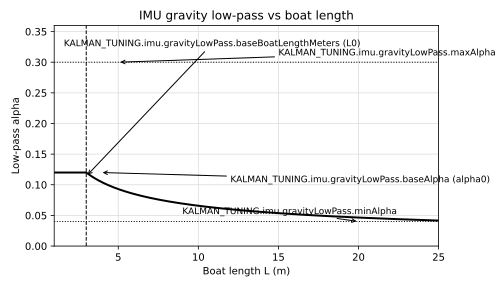
\includegraphics{./plots/gain-gravity-alpha.pdf}
\caption{IMU gravity low-pass vs boat length}
\end{figure}

\hypertarget{process-noise-anisotropy-forward-vs-lateral}{%
\subsection{Process noise anisotropy (forward vs
lateral)}\label{process-noise-anisotropy-forward-vs-lateral}}

Boats change speed much more easily along their heading than sideways.
We encode that by scaling the lateral acceleration variance as a fixed
fraction of the forward variance:

\[
q_{\text{lateral}} = \rho\,q_{\text{forward}}
\]

Variables:
in code, \(\rho\) is \texttt{KALMAN\_TUNING.imu.lateralVarianceRatio}.

\clearpage
\part{RaceVMG}
\noindent This part covers RaceVMG (VMG Hunter): how we estimate the local speed--heading
trade-off upwind (without a wind sensor), what we can and cannot infer from GPS alone,
and how that estimate is presented in a way that makes steering decisions feel natural.
% !TeX root = master.tex

\section{RacePerformance (VMG evaluator)}

This section describes how RacePerformance turns a stream of heading and speed samples into a
simple, stable evaluation: how much the most recent behavior improves or degrades VMG
relative to a low-pass baseline. The goal is not to estimate true wind, but to provide a
consistent reference so changes in trim or steering show up as a clear percentage.

\subsection{Signals and baseline filters}

This subsection defines the signals used by the evaluator and how they are filtered.

RacePerformance applies a first-order low-pass baseline and computes deviations:
\begin{flalign}
\hspace{5em}\alpha_k &= \frac{\Delta t_k}{\tau+\Delta t_k} && \left[1\right] \label{eq:vmg:alpha}
\end{flalign}
In \eqref{eq:vmg:alpha}, \(\alpha_k\) is the per-sample gain, \(\Delta t_k\) is the sample
interval, the subscript \(k\) is the sample index, and \(\tau\) is the user-selected time
constant. This gain is applied to the speed baseline in the next step.
\begin{flalign}
\hspace{5em}\overline{v}_k &= \overline{v}_{k-1}+\alpha_k\left(v_k-\overline{v}_{k-1}\right) && \left[\text{m/s}\right] \label{eq:vmg:vbar-update}
\end{flalign}
In \eqref{eq:vmg:vbar-update}, \(v_k\) is the instantaneous boat speed from the Kalman
state, optionally enhanced by the device motion sensor, and \(\overline{v}_k\) is the
low-pass speed baseline. The same gain is then applied to heading with angular wrap.
\begin{flalign}
\hspace{5em}\overline{h}_k &= \overline{h}_{k-1}+\alpha_k\,\mathrm{wrap}\left(h_k-\overline{h}_{k-1}\right) && \left[\text{rad}\right] \label{eq:vmg:hbar-update}
\end{flalign}
In \eqref{eq:vmg:hbar-update}, \(h_k\) is the instantaneous heading, \(\overline{h}_k\) is
the baseline heading, and \(\mathrm{wrap}(\cdot)\) returns the shortest signed angular
difference. The filters start from the first sample to avoid a delayed plot.
\begin{flalign}
\hspace{5em}\overline{v}_0 &= v_0 && \left[\text{m/s}\right] \label{eq:vmg:vbar-init}
\end{flalign}
In \eqref{eq:vmg:vbar-init}, the subscript \(0\) denotes the first sample used to
initialize the speed baseline. The heading baseline is initialized in the same way.
\begin{flalign}
\hspace{5em}\overline{h}_0 &= h_0 && \left[\text{rad}\right] \label{eq:vmg:hbar-init}
\end{flalign}
In \eqref{eq:vmg:hbar-init}, the first heading sample anchors the baseline. With
baselines defined, we compute the deviations.
\begin{flalign}
\hspace{5em}\Delta v_k &= v_k-\overline{v}_k && \left[\text{m/s}\right] \label{eq:vmg:dv}
\end{flalign}
In \eqref{eq:vmg:dv}, \(\Delta v_k\) is the speed deviation from the baseline. The
heading deviation follows.
\begin{flalign}
\hspace{5em}\Delta h_k &= \mathrm{wrap}\left(h_k-\overline{h}_k\right) && \left[\text{rad}\right] \label{eq:vmg:dh}
\end{flalign}
In \eqref{eq:vmg:dh}, \(\Delta h_k\) is the signed heading deviation, wrapped to the
shortest angular difference. The derivation below omits the sample index for clarity.
The evaluator is driven by the same Kalman output stream as the track view, so it updates
on prediction steps as well as GPS updates.

\subsection{VMG improvement model}
This subsection explains how mode, tack, and the assumed TWA enter the percent-improvement
calculation. It starts by defining the tack-signed target angle, then defines VMG, and
finally derives the improvement expression and its mode-specific forms.

\begin{flalign}
\hspace{5em}a &=
\begin{cases}
-a_{\mathrm{up}}, & \text{beat, port tack} \\
\phantom{-}a_{\mathrm{up}}, & \text{beat, starboard tack} \\
0, & \text{reach mode} \\
-a_{\mathrm{down}}, & \text{run, port tack} \\
\phantom{-}a_{\mathrm{down}}, & \text{run, starboard tack}
\end{cases}
&& \left[\text{rad}\right] \label{eq:vmg:target-angle}
\end{flalign}
In \eqref{eq:vmg:target-angle}, \(a\) is the signed target TWA, \(a_{\mathrm{up}}\) is
the upwind target, and \(a_{\mathrm{down}}\) is the downwind target. Port uses the
negative sign and starboard uses the positive sign. With \(a\) fixed, we define the
baseline VMG.
Reach mode deserves an explicit interpretation. In \eqref{eq:vmg:target-angle} we set
\(a=0\) for reach, which makes the improvement measure track how well you hold the
baseline direction rather than true wind progress. That is a stretch to call VMG: it
assumes you want to keep going where you are going on average, and any deviation from
that baseline is treated as under-performance.
\begin{flalign}
\hspace{5em}\overline{w} &= \overline{v}\cos a && \left[\text{m/s}\right] \label{eq:vmg:wbar}
\end{flalign}
In \eqref{eq:vmg:wbar}, \(\overline{w}\) is the baseline VMG and \(\overline{v}\) is the
low-pass speed baseline. The instantaneous VMG uses the current speed and heading
deviation.
\begin{flalign}
\hspace{5em}w &= v\cos\left(a+\Delta h\right) && \left[\text{m/s}\right] \label{eq:vmg:w}
\end{flalign}
In \eqref{eq:vmg:w}, \(w\) is the instantaneous VMG, \(v\) is the instantaneous speed,
and \(\Delta h\) is the heading deviation. The improvement ratio compares instantaneous
to baseline VMG.
\begin{flalign}
\hspace{5em}R &= \frac{w}{\overline{w}} && \left[1\right] \label{eq:vmg:ratio}
\end{flalign}
In \eqref{eq:vmg:ratio}, \(R\) is the VMG ratio. With \(R\) defined, we convert the ratio
to a percentage before returning it to the UI.
\begin{flalign}
\hspace{5em}\eta &= 100\left(R-1\right) && \left[\%\right] \label{eq:vmg:eta}
\end{flalign}
In \eqref{eq:vmg:eta}, \(\eta\) is the percent improvement shown in the UI. The mode
choice only selects the target angle \(a\) using \eqref{eq:vmg:target-angle}: reach sets
\(a=0\), beat uses the upwind target with a negative sign on port and a positive sign on
starboard, and run uses the downwind target with the same sign rule. In run mode the
target angle exceeds ninety degrees, so the cosine term is negative; both baseline and
instantaneous VMG share that sign, and the ratio still reports a positive improvement for
faster or better-aligned running.

\subsection{Displayed signal and plot window}

This subsection describes the optional smoothing of the displayed signal and how the time
history window is chosen.

The baseline filters always use the long time constant chosen by the user. The displayed
signal can either be the raw improvement or a ``fast'' smoothed version that uses a
shorter time constant.
\begin{flalign}
\hspace{5em}\tau_{\mathrm{fast}} &= \frac{\tau}{10} && \left[\text{s}\right] \label{eq:vmg:tau-fast}
\end{flalign}
In \eqref{eq:vmg:tau-fast}, \(\tau_{\mathrm{fast}}\) is used only for the display; the
baseline filters remain set by \(\tau\). If the baseline magnitude is too small, the
output is suppressed until it stabilizes.

The plot window length is defined by the main time constant.
\begin{flalign}
\hspace{5em}T_{\mathrm{window}} &= 2\tau && \left[\text{s}\right] \label{eq:vmg:window}
\end{flalign}
In \eqref{eq:vmg:window}, \(T_{\mathrm{window}}\) is the fixed plot span of two time
constants. The time axis
runs left to right with ``now'' at the right edge. We draw the improvement history as a
line with a filled area underneath: green for positive values and red for negative
values. The percent axis is symmetric with labeled ticks. An optional cap limits the
displayed magnitude to a fixed percentage so outliers do not rescale the plot.

\subsection{Heading sources and device motion}

This subsection describes how heading is sourced and how the device motion option
interacts with GPS.

RacePerformance always uses the Kalman heading. When the device motion sensor is enabled, we
integrate yaw rate to track
short-term heading changes and blend it back toward GPS heading when speed is sufficient
and accuracy is acceptable. This improves responsiveness when the phone is rigidly
mounted to the boat, but it can degrade estimates if the phone is hand-held or moved
relative to the boat, which is why the UI warns about mounting.

\clearpage
\appendix
% !TeX root = master.tex

\section{Appendix}

\subsection{Coordinate system: latitude/longitude to meters}

Internally, the filter runs in a local tangent-plane approximation:
\begin{itemize}
\tightlist
\item
  choose a local origin near the current area
\item
  convert \((\text{lat}, \text{lon})\) into \((x, y)\) meters relative to that origin
\end{itemize}

This is implemented with helpers in \texttt{geo.js} (\texttt{toMeters}, \texttt{fromMeters}).
Over the distances we care about at a start line, this approximation is accurate enough and
avoids complicated geodesy inside the filter.


\end{document}
